\documentclass[11pt]{article}
\usepackage[letterpaper,margin=1in]{geometry}
\usepackage[T1]{fontenc}
\usepackage{lmodern,microtype}
\usepackage{amsmath,amssymb,booktabs,array,longtable}
\PassOptionsToPackage{svgnames}{xcolor}
\usepackage{graphicx,xcolor,tikz}
\usepackage{caption}
\usepackage[numbers,sort&compress]{natbib}
\usepackage[colorlinks=true,allcolors=blue!45!black,breaklinks=true]{hyperref}
\hypersetup{pdftitle={LegalForecastBench: Forecasting Judicial Decisions as a Test of Legal Reasoning Ability},pdfauthor={John J. Hughes, III},pdfsubject={Legal forecasting, probabilistic evaluation, and outcome feedback},pdfkeywords={legal AI, forecasting, benchmark, Brier score, reinforcement learning}}
\urlstyle{same}
\captionsetup{font=small,labelfont=bf}
% Drafting markers. A line starting with % TODO is visible only in the source.
% \todo prints a margin note; \todo[inline] prints a note in the text.
% Colored macros mark provisional prose. For a clean PDF, load todonotes as
% \usepackage[disable]{todonotes} and redefine \draft, \checkcite, and \checknum
% to return their argument unchanged.
\usepackage{todonotes}
\newcommand{\draft}[1]{\textcolor{red}{#1}}
\newcommand{\checkcite}[1]{\textcolor{blue}{#1}}
\newcommand{\checknum}[1]{\textcolor{orange}{#1}}
\setlength{\emergencystretch}{2em}
% Flush paragraphs. A gap marks a new paragraph; no line is indented.
\usepackage[skip=0.6em]{parskip}
\title{LegalForecastBench: Forecasting Judicial Decisions\\as a Test of Legal Reasoning Ability}
\author{John J. Hughes, III\\Independent researcher\\\url{https://www.johnjhughes3.com/research/}}
\date{Working paper --- September 29, 2026}
\begin{document}
\maketitle
\begin{abstract}
% TODO: revise the abstract at the end, after the rest of the paper is settled
\draft{Legal AI evaluations increasingly assess professional work products with expert-written rubrics. Judicial forecasting offers a complementary target: an uncertain legal judgment whose realized outcome can subsequently be observed. We introduce LegalForecastBench, a benchmark of claim--defendant-level dismissal probabilities from pre-decision records in U.S. federal litigation. The beta contains 91 cases decided between June 30 and August 7, 2026, with 387 scored units. In a fixed panel of twelve document-enabled model configurations, GPT-6 Sol has the lowest observed micro-Brier loss (0.11763) and the highest unit accuracy (84.50\%). All twelve improve on a retrospectively fitted constant-probability reference; eleven improve on majority-class accuracy. Confidence differs substantially across configurations, and several strong models make consequential high-confidence errors. In a separate shared-summary experiment, two Luna configurations substantially outperform Jev; Jev underpredicts dismissal in the aggregate. We distinguish these evaluation findings from the hypothesis that outcome feedback can improve legal judgment, describe LegalForecastGym as a setting for testing that hypothesis, and examine task--rubric alignment through a bounded case study of Harvey's Legal Agent Benchmark. The contribution is a legally specified probabilistic evaluation task and empirical baseline, with explicit limits concerning label adjudication, selection, contamination, repeated-run uncertainty, and transfer beyond forecasting.}
\end{abstract}

\section{Introduction}
Reinforcement learning (RL) techniques have led to significant recent gains in the reasoning abilities of frontier AI models, particularly on verifiable tasks. RL training environments specify what a model can observe and do, and which outcomes receive reward. In \emph{reinforcement learning with verifiable rewards} (RLVR), correctness checks (like mathematical answer matching, executable tests, or formal proof checking) supply a scalable training signal that does not require a human to assess every model response \citep{deepseek,rlve}. Earlier self-play systems demonstrated the power of outcome feedback in games with explicit rules \citep{alphazero}.

The efficiacy of these techniques in verifiable domains has been exceptional. During reinforcement learning, DeepSeek-R1-Zero's average pass@1 on AIME 2024 rose from 15.6\% to 77.9\%; the final DeepSeek-R1 system, which used a broader training pipeline, reached the 96.3rd percentile on Codeforces \citep{deepseek}. AlphaProof coupled reinforcement learning with Lean's formal proof checker and proved three problems from the 2024 International Mathematical Olympiad, including its hardest problem, solved by only five of 609 human contestants \citep{alphaproof}. And OpenAI's September 2026 announcement that it had solved the Navier--Stokes Millennium Prize Problem reportedly relied on an internal model developed through large-scale reinforcement learning, followed by Lean formalization and verification. \citep{navierstokesproof,navierstokesreport}. While the training methods  used in some systems that have achieved recent breakthroughs are not fully public, and technques other than verficiation and reinforcement learning likely contributed, the results illustrate the enormous, often superhuman, capabilities that frontier models have obtained in verifiable domains, in signiciant part through reinforcement learning.

Open-ended professional legal tasks are often considered nonverifiable and are therefore less susceptible to the RLVR techniques that have proved effective in domains like mathematics and coding. Many legal tasks involve questions of judgment on which there are several potentially defensible answers, and there is no automated way to determine which is best. Two approaches that have been proposed are preference evaluation (comparing which of two outputs practicing attorneys prefer) and rubric-based reinforcement learning (grading model outputs against specified criteria to produce a reward). \citep{judgmentbench}. \emph{Rubrics as Rewards} studies this approach in medicine and science \citep{rubricsrewards}, and leading vertical AI companies such as Harvey AI Corporation (Harvey) have started using rubric-based rewards to train models for legal use. \citep{harveyTraining,tenet}. These techniques do not supply human-written demonstrations for supervised training \citep{instructgpt}. Instead, the rubric defines what the system is rewarded for doing, and separate LLMs can judge the outputs against the rubric to produce a reward.

Rather than treat legal strictly as a nonverifiable domain, legal tasks may be more accurately understood as lying on a spectrum. Some legal propositions are settled, bright-line rules that can be tested objectively;

Legal tasks are more accurately understood as lying on a spectrum. Some questions can be checked against settled rules and specified facts; others turn on standards or interpretations about which reasonable lawyers can disagree. LegalBench, for example, deliberately focuses on tasks with unambiguous answers \citep{legalbench}. The Multistate Bar Examination illustrates the first kind of evaluation: it tests the application of fundamental legal principles to given facts and scores answers against a key \citep{ncbe}. Hart's classic example illustrates how uncertainty can arise even under a short rule: a prohibition on vehicles in a park clearly covers automobiles, but its application to bicycles or toy cars is less certain \citep{hart}. Fuller's reply asks whether the same rule would prohibit a military truck displayed as a war memorial, illustrating the role of purpose and context \citep{fuller}.

Litigation provides a mechanism for resolving that uncertainty. Before a contract dispute is adjudicated, lawyers for each side may disagree about what the contract means or whether a contemplated action would breach it. A judgment resolving those questions determines the parties' rights, subject to appeal and the rules governing finality. The Declaratory Judgment Act expressly permits a court with jurisdiction over an actual controversy to declare those rights with the force of a final judgment \citep{declaratory}. An erroneous judgment can still have binding consequences \citep{moitie}. Litigation thus turns a disputed question into an observable, legally operative disposition. It need not make the court's reasoning indisputably correct or settle the law for everyone.

A legal question need not have an uncontested correct answer to support a forecast scored against a court's eventual decision. Once the forecast event is specified and the disposition reliably labeled, a proper scoring rule supplies a reproducible score. A single outcome does not verify an individual probability estimate; proper scores encourage truthful reporting in expectation, and calibration is assessed across forecasts \citep{brier,gneiting}. Mapping decisions to claim-level labels still requires legal judgment. The event itself need not be final or irreversible: LegalForecastBench targets the motion's first written disposition.

The connection between legal judgment and prediction is longstanding. Holmes placed prediction of what courts will do at the center of the lawyer's practical task \citep{holmes}. Mnookin and Kornhauser's account of bargaining in the shadow of the law explains why expected judicial outcomes influence negotiations even when the parties never go to court. Their custody example makes the point concrete: the best-interests-of-the-child standard leaves considerable uncertainty about a judge's decision, yet assessments of the likely outcome and attitudes toward risk still shape bargaining \citep{shadow}. The probabilities concern specified judicial outcomes, without requiring an intrinsic numerical probability for every contested proposition of law.

\textbf{LegalForecastBench} is an effort to apply this property of litigation to the evaluation of frontier AI models and to investigate a potential source of training signal. Predicting how a dispute will be resolved is an important judgment task in litigation practice. A lawyer advising a client must understand the client's goals, analyze the facts and applicable law, assess the counterparty's incentives, and develop a strategy for obtaining an achievable outcome. Prediction is one component of that work, but it influences several others: which arguments to emphasize, what risks to communicate, and what negotiated resolution to accept \citep{nylawyerskills,shadow}. Section~\ref{sec:strategy} develops these connections. The value of prediction therefore extends beyond forecasting cases that ultimately reach judgment.

We collected 91 real matters with written decisions on motions to dismiss. A mixed-model pipeline with human legal oversight identified the challenged claims and moving defendants and labeled the resulting dispositions. The evaluation contains 387 scored claim--defendant units, each representing a challenged claim against one defendant or a group treated together on materially identical grounds. Models receive the pre-decision record and predict the probability that each unit will be dismissed in full in the motion's first written disposition. The headline metric is micro-Brier loss, a proper score for probabilistic forecasts. GPT-6 Sol had the best observed scores, but this small, single-retained-run comparison is intended primarily to establish the framework, not a general model hierarchy. A separate experiment tests whether a compact probabilistic model can use summaries of the same records.

The benchmark is motivated by the ability to distinguish facts and arguments that matter to an outcome. Its score directly measures forecast performance; it does not establish that a model identified the decisive issue or reasoned correctly. The training hypothesis is related but separate. Just as next-token prediction can induce representations useful beyond the immediate prediction task, predicting litigation outcomes may help models learn which facts, legal rules, and procedural constraints influence judicial decisions. Outcome-based forecasting research supplies precedents for this direction \citep{outcomerl,openforecaster,sentencing}. LegalForecastGym provides a setting for testing it. Whether improvements transfer to legal advice or strategy remains an empirical question.

As part of this work, we also examine rubric-based evaluation through a preliminary audit of Harvey's Legal Agent Benchmark and a detailed review of one litigation task. The review identifies ways in which a fictional record, its legal criteria, and the requested work product can diverge \citep{labaudit,labtask}. This raises a question of \emph{construct validity}: whether the score adequately represents the professional capability being evaluated \citep{jacobswallach}. When those criteria supply training rewards, the corresponding concern is \emph{reward misspecification}. Work on reward-model overoptimization shows why optimizing a proxy more successfully need not improve the underlying objective \citep{amodei,gao}. Our audit does not establish that fictitious environments or rubric-based RL are ineffective. It motivates comparing carefully specified rewards and authentic litigation outcomes, while recognizing the limitations of both.

\section{Related work}
\paragraph{Legal outcome prediction.} Judicial prediction predates large language models. Ruger and colleagues compared statistical and expert forecasts of Supreme Court decisions, and Katz, Bommarito, and Blackman developed a general approach to predicting Supreme Court behavior over a long historical period \citep{ruger,katz}. Text-based prediction of European Court of Human Rights decisions and large Chinese judgment datasets broadened the field \citep{aletras,cail}. These tasks differ in jurisdiction, information set, granularity, and whether inputs are written before or as part of the judgment. Medvedeva and McBride emphasize that predicting labels from judicially authored accounts can diverge sharply from the information available to a real forecaster \citep{medvedeva}. CLC-UKET is a particularly relevant comparison that includes human predictions, but its facts and claims are extracted from judgments; the authors identify original party submissions as an important next step \citep{clcuket}. Commercial motion-prediction products also exist. We therefore make no claim to the first judicial, U.S., or motion-to-dismiss predictor. Our specific object is a refreshable, probabilistically scored, claim--defendant-level evaluation using the pre-decision written record.

\paragraph{Professional legal evaluation.} LegalBench organizes legal reasoning tasks around domain expertise \citep{legalbench}. LAB assesses document- and tool-based legal assignments with detailed criteria, while JudgmentBench compares rubric and preference evaluation on constructed quality levels in a different legal benchmark, BigLaw Bench \citep{harveyLAB,judgmentbench}. Forecasting and work-product evaluation measure different constructs. An excellent opposition memorandum can lose; a poor memorandum can prevail for reasons unrelated to its quality. Outcome forecasting complements evaluation of legal work products and cannot replace it.

\paragraph{Verification, rewards, and forecasting.} Rule-based rewards, learned preferences, and process supervision supply different forms of training feedback \citep{deepseek,lightman,instructgpt}. Autocast established a substantial real-world event-forecasting dataset, and Halawi and colleagues combined retrieval, reasoning, and fine-tuning for forecasting \citep{autocast,halawi}. Outcome-based reinforcement learning and OpenForecaster train using resolved events \citep{outcomerl,openforecaster}; ForecastBench uses evolving real-world questions to address contamination and evaluate forecasting \citep{forecastbench}. Chinese sentencing work combines outcome-related rewards with intermediate reasoning assessment \citep{sentencing}. These are direct antecedents of the proposed learning direction. None, by itself, establishes that training on U.S. motion outcomes improves broader litigation judgment.

\paragraph{Measurement validity.} Proper scoring rules encourage honest probabilities in expectation \citep{brier,gneiting}. Statistical evaluation must also respect dependence among questions sharing a record \citep{miller}. Real-world provenance does not eliminate specification error: SWE-bench's executable tests and subsequent analyses illustrate the need to align the task, information supplied, and criterion of success \citep{swebench,swecritique}. The same alignment problem applies both to legal rubrics and to our own outcome labels.

\section{Dataset and task}
\subsection{Prediction target and information set}
Let $c\in\{1,\ldots,C\}$ index cases and $u\in\mathcal U_c$ index scored units within case $c$. Each unit identifies a challenged claim or independently disposable pleaded subclaim against a moving defendant or a group treated together on materially identical grounds. A legal defense, claim element, requested remedy, or factual theory is not automatically a separate unit. The model receives the pre-decision record $X_c$ and unit specification $U_{cu}$ and returns
\begin{equation}
 p_{cu}\in[0,1],\qquad p_{cu}\approx \Pr(Y_{cu}=1\mid X_c,U_{cu}),
\end{equation}
where $Y_{cu}=1$ means full dismissal of that unit in the target motion's first written disposition. The event is not final victory in the lawsuit.

A full dismissal with leave to amend still has label 1. A partial dismissal that leaves the frozen unit alive in a material respect has label 0. Later amendment, settlement, reconsideration, and appellate reversal do not retroactively change this target. Dispositions that cannot be reliably mapped to the unit are excluded from primary scoring. These choices sacrifice some procedural detail for a stable, interpretable forecast event. They also make label construction a legal task in its own right.

\begin{table}[ht]
\centering\small
\begin{tabular}{p{.60\linewidth}p{.29\linewidth}}
\toprule
First written disposition of the frozen unit & Primary label \\
\midrule
Entire claim dismissed, with or without leave to amend & $1$: fully dismissed \\
Only one nonseparable theory or remedy dismissed; claim remains & $0$: not fully dismissed \\
Claim dismissed against one defendant but survives against another & Separate labels for separately frozen units \\
Disposition does not reliably resolve the frozen target & Excluded from primary scoring \\
\bottomrule
\end{tabular}
\caption{Illustrative label semantics, not additional dataset observations. The documented protocol defines unit boundaries before consulting the outcome.}
\label{tab:labels}
\end{table}

\subsection{Cohort construction and labeling}
The analyzed release contains 91 U.S. federal cases with written decisions dated June 30--August 7, 2026. The retained package contains 409 forecast units, of which 387 are scored; 22 units therefore do not enter the headline metrics. Of the scored units, 285 were fully dismissed and 102 were not. The shared-summary preparation inventory contains 482 selected documents. We report the analyzed cohort rather than implying a random sample of all federal motions. The materials reviewed for this paper do not provide a complete population-level sampling frame or a reason-by-reason census of every excluded acquisition candidate.

The documented construction pipeline combines models with human legal oversight. Its protocol identifies units from pre-decision material and uses a separate stage to interpret the subsequent disposition for those frozen targets. The documented labeling policy requires structured outcome agreement and supporting disposition excerpts for automatic acceptance, with disagreement, ambiguity, and structural defects routed to lawyer review. The author reports resolving disputed units and correcting labels. This is not a completed independent label-error study: this paper does not report an adjudication rate, inter-annotator agreement, or a blinded human-audit error estimate. Current pipeline documentation also contains later refinements and should not be mistaken for a census of the operations performed on every historical beta case.

The important separation is between \emph{unitization} and \emph{outcome coding}. A decision must not be used to invent a prediction unit after the fact. Conversely, an expressly pleaded but legally defective claim is still a potential forecast target if the motion challenges it; deciding that the claim lacks legal merit is not a reason to remove it from the task. Authentic litigation records require this distinction because pleadings, motions, and dispositions rarely share a perfectly aligned schema.


\begin{figure}[tb]
\centering
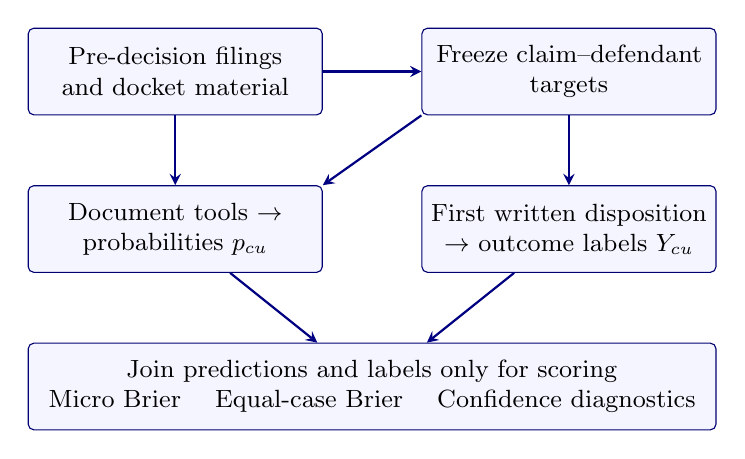
\begin{tikzpicture}[every node/.style={font=\small,align=center},box/.style={draw=blue!45!black,rounded corners=2pt,fill=blue!4,text width=3.5cm,minimum height=1.1cm},arr/.style={->,>=stealth,thick,draw=blue!50!black}]
\node[box] (record) at (0,0) {Pre-decision filings\\and docket material};
\node[box] (units) at (5,0) {Freeze claim--defendant\\targets};
\node[box] (forecast) at (0,-2) {Document tools $\rightarrow$\\probabilities $p_{cu}$};
\node[box] (outcome) at (5,-2) {First written disposition\\$\rightarrow$ outcome labels $Y_{cu}$};
\node[box,text width=8.5cm] (score) at (2.5,-4) {Join predictions and labels only for scoring\\Micro Brier \quad Equal-case Brier \quad Confidence diagnostics};
\draw[arr] (record)--(units);
\draw[arr] (record)--(forecast);
\draw[arr] (units) -- (outcome);
\draw[arr] (units.south west)--(forecast.north east);
\draw[arr] (forecast)--(score);
\draw[arr] (outcome)--(score);
\end{tikzpicture}
\caption{Information separation in the forecasting task. Models inspect pre-decision material and frozen targets. The subsequent judicial disposition is used in the labeling and scoring path, not in the model-visible packet. In the retrospective beta, this is an information boundary rather than a claim that forecasts were made before the decisions occurred.}
\label{fig:pipeline}
\end{figure}


\subsection{Temporal design and contamination}
The target decision and its outcome are withheld from the model-visible record. Packet construction screens docket and filing text for outcome leakage. The model-visible document-tool sandbox provides no Internet research access; provider transport remains available. These measures control the supplied information, not the model's pretraining or post-training history.

The decision window follows the reported knowledge or training cutoffs for nine configurations under the repository's maintained eligibility rule. Fable's month-only June 2026 cutoff can overlap the earliest decision; Kimi and Muse have no established cutoff in the retained evidence. Knowledge cutoffs are provider statements and need not describe every training exposure. Model release dates are not substitutes for training-data dates. Appendix~\ref{app:cutoffs} makes this distinction explicit. The appropriate description is \emph{historical temporal holdout with qualified contamination resistance}, not proof that all evaluated models were unexposed.

The acquisition and labeling pipeline is designed to issue later cohorts as new decisions become available. This enables fresh comparisons after earlier benchmark data become public. A genuinely prospective evaluation would freeze predictions before the judicial outcomes occur; the present beta is retrospective. Refreshing a benchmark also changes its case mix and difficulty. Scores from different versions should not be interpreted as a time series of model improvement without common comparators and appropriate adjustment.

\section{Evaluation protocol and scoring}
\subsection{Execution}
The main comparison uses a common document-access interface for the full pre-decision packet, with model-provider access and no Internet research. Models can inspect documents through tools and produce a probability for each unit, together with a short rationale. Provider-specific reasoning settings are retained in the run registries; a common interface does not imply identical inference budgets or identical serving behavior. Appendix~\ref{app:protocol} lists the configuration settings.

The beta retains one successful forecast for each configuration and unit. Recovery completed interrupted or failed cases, but the analysis does not measure first-attempt completion probability, failure-adjusted utility, or run-to-run variance. The main panel is fixed to the twelve configurations in the source draft; later repository additions do not silently change the study population. Numerical results are checked against retained aggregates, and available unit-level exports are recomputed separately.

\subsection{Proper scores and descriptive references}
For $N=\sum_c |\mathcal U_c|=387$ and $C=91$, the primary metric is the micro-Brier loss
\begin{equation}
 B_{\mathrm{micro}}=\frac{1}{N}\sum_{c=1}^C\sum_{u\in\mathcal U_c}(p_{cu}-Y_{cu})^2.
\label{eq:micro}
\end{equation}
The equal-case score changes the estimand by giving each case the same weight:
\begin{equation}
 B_{\mathrm{case}}=\frac{1}{C}\sum_{c=1}^C\frac{1}{|\mathcal U_c|}\sum_{u\in\mathcal U_c}(p_{cu}-Y_{cu})^2.
\label{eq:case}
\end{equation}
Both are lower-is-better. Micro-Brier emphasizes the experience of a scored claim--defendant unit; equal-case Brier reduces the influence of cases containing many units. Neither score should be selected after looking at which gives a preferred model ordering.

The Brier rule is strictly proper for the binary target. If the true conditional event probability is $q$, then
\begin{equation}
 \mathbb E[(p-Y)^2\mid X,U]=(p-q)^2+q(1-q),
\label{eq:proper}
\end{equation}
which is minimized by reporting $p=q$. The second term is irreducible uncertainty for that information set. An observable judicial event therefore supports a verifiable score, although one realized outcome cannot reveal whether an individual probability was correct \citep{brier,gneiting}.

We report accuracy at threshold $p\geq0.5$ as a secondary descriptive metric. The observed dismissal frequency is $\widehat\pi=285/387=0.73643$. A constant forecast $p=\widehat\pi$ has micro-Brier $\widehat\pi(1-\widehat\pi)=0.19410$; always predicting dismissal has accuracy 73.64\%. The constant is fitted retrospectively on this cohort, so it is a descriptive reference, not a deployable baseline trained on earlier cases. The uninformative forecast $p=0.5$ has Brier 0.25. A random hard classification is a different baseline and should not be conflated with a probability of one-half.

Log loss is a complementary diagnostic:
\begin{equation}
 L=-\frac{1}{N}\sum_{c,u}\left[Y_{cu}\log p_{cu}+(1-Y_{cu})\log(1-p_{cu})\right].
\end{equation}
For a wrong forecast assigning 0.99 to the predicted class, Brier loss is 0.9801 and log loss is approximately 4.605; at confidence 0.90 the corresponding losses are 0.81 and 2.303. Thus log loss places a particularly large penalty on extreme errors. A complete twelve-model log-loss table is unavailable: unit-level data sufficient to rederive it were available for only five main-panel configurations in the checked local export.

\subsection{Uncertainty and scope of inference}
Units within the same case share facts and outcomes. The historical ten-configuration analysis used a paired case-cluster percentile bootstrap with one million resamples, correcting across 45 model pairs and three metrics. Its retained summary reports only three distinguishable comparisons, all involving worse scores for Muse: against Grok 4.6 on both Brier metrics and against Opus 5 on micro-Brier. This does not establish equivalence among the other models.

The expanded twelve-configuration table is descriptive. We do not attach the historical significance statements to GPT-6 Sol or Grok 4.7. Seven of the original twelve configurations lack locally retained unit-level inputs in the checked site export, preventing a complete reanalysis from that export. The shared-summary experiment has its own complete three-condition comparison and its own multiplicity correction. Neither analysis establishes independence across related cases or multidistrict-litigation families, and neither measures variation across repeated model runs \citep{miller}.

\section{Results}
\subsection{Full-document comparison}
Table~\ref{tab:main} reports the fixed twelve-configuration panel. GPT-6 Sol achieves the best observed micro-Brier (0.11763), equal-case Brier (0.12949), and accuracy (327/387, 84.50\%). Relative to the retrospectively fitted constant, its micro-Brier is lower by about 39.4\%. All twelve configurations beat that Brier reference; eleven beat majority-class accuracy. Muse's 279/387 correct forecasts (72.09\%) illustrate why accuracy and probability quality need not give the same comparison.

\begin{table}[tb]
\centering\small
\setlength{\tabcolsep}{4pt}
\begin{tabular}{lrrrrr}\toprule
Configuration & Micro Brier & Case Brier & Correct & Acc. (\%) & Cost (\$)\\\midrule
GPT-6 Sol & 0.11763 & 0.12949 & 327/387 & 84.50 & 11.01 \\
Claude Fable 5.1 & 0.12877 & 0.13653 & 318/387 & 82.17 & 83.18 \\
Grok 4.6 & 0.13368 & 0.13480 & 312/387 & 80.62 & 15.72 \\
Claude Opus 5 & 0.13987 & 0.13548 & 310/387 & 80.10 & 45.89 \\
GPT-5.6 Sol & 0.14009 & 0.13319 & 313/387 & 80.88 & 24.91 \\
Kimi K3 & 0.14130 & 0.15367 & 303/387 & 78.29 & 16.87 \\
GPT-5.6 Luna & 0.14322 & 0.15084 & 313/387 & 80.88 & 1.48 \\
GPT-6 Astra & 0.15221 & 0.14275 & 305/387 & 78.81 & 59.74 \\
Gemini 3.8 Flash & 0.15331 & 0.13900 & 310/387 & 80.10 & 35.61 \\
Grok 4.7 & 0.15833 & 0.16454 & 298/387 & 77.00 & 33.00 \\
Claude Sonnet 5 & 0.15848 & 0.15964 & 293/387 & 75.71 & 24.68 \\
Muse Spark 1.3 & 0.18121 & 0.17845 & 279/387 & 72.09 & 8.78 \\
\midrule
Cohort-rate reference & 0.19410 & --- & 285/387 & 73.64 & ---\\
Constant $p=0.5$ & 0.25000 & 0.25000 & --- & --- & ---\\
\bottomrule\end{tabular}
\caption{Full-document results, ordered by micro-Brier loss. Each model row covers 91 cases and 387 scored units. The last column reports the retained successful-workload cost estimate under heterogeneous accounting assumptions detailed in the text; it is not a controlled price comparison. The cohort-rate reference is retrospectively fitted, and its accuracy column uses always-dismiss classification. No twelve-model significance ordering is claimed.}
\label{tab:main}
\end{table}

\begin{figure}[tb]\centering
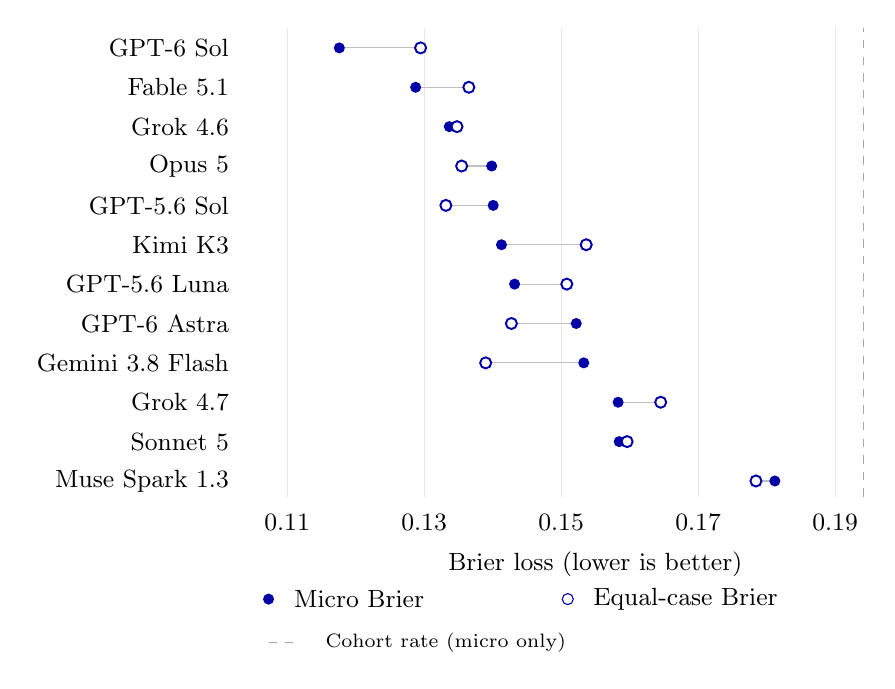
\begin{tikzpicture}[every node/.style={font=\small}]
\draw[gray!18] (0.43500,-.2)--(0.43500,5.750);
\node[anchor=north] at (0.43500,-.3) {0.11};
\draw[gray!18] (2.17500,-.2)--(2.17500,5.750);
\node[anchor=north] at (2.17500,-.3) {0.13};
\draw[gray!18] (3.91500,-.2)--(3.91500,5.750);
\node[anchor=north] at (3.91500,-.3) {0.15};
\draw[gray!18] (5.65500,-.2)--(5.65500,5.750);
\node[anchor=north] at (5.65500,-.3) {0.17};
\draw[gray!18] (7.39500,-.2)--(7.39500,5.750);
\node[anchor=north] at (7.39500,-.3) {0.19};
\draw[dashed,gray!70] (7.75160,-.2)--(7.75160,5.750);
\node[anchor=east] at (-.18,0.000) {Muse Spark 1.3};
\draw[gray!50] (6.62998,0.000)--(6.38993,0.000);
\fill[blue!65!black] (6.62998,0.000) circle (2pt);
\draw[blue!65!black,fill=white,line width=.7pt] (6.38993,0.000) circle (2pt);
\node[anchor=east] at (-.18,0.500) {Sonnet 5};
\draw[gray!50] (4.65311,0.500)--(4.75361,0.500);
\fill[blue!65!black] (4.65311,0.500) circle (2pt);
\draw[blue!65!black,fill=white,line width=.7pt] (4.75361,0.500) circle (2pt);
\node[anchor=east] at (-.18,1.000) {Grok 4.7};
\draw[gray!50] (4.63933,1.000)--(5.18010,1.000);
\fill[blue!65!black] (4.63933,1.000) circle (2pt);
\draw[blue!65!black,fill=white,line width=.7pt] (5.18010,1.000) circle (2pt);
\node[anchor=east] at (-.18,1.500) {Gemini 3.8 Flash};
\draw[gray!50] (4.20331,1.500)--(2.95760,1.500);
\fill[blue!65!black] (4.20331,1.500) circle (2pt);
\draw[blue!65!black,fill=white,line width=.7pt] (2.95760,1.500) circle (2pt);
\node[anchor=east] at (-.18,2.000) {GPT-6 Astra};
\draw[gray!50] (4.10730,2.000)--(3.28403,2.000);
\fill[blue!65!black] (4.10730,2.000) circle (2pt);
\draw[blue!65!black,fill=white,line width=.7pt] (3.28403,2.000) circle (2pt);
\node[anchor=east] at (-.18,2.500) {GPT-5.6 Luna};
\draw[gray!50] (3.32487,2.500)--(3.98765,2.500);
\fill[blue!65!black] (3.32487,2.500) circle (2pt);
\draw[blue!65!black,fill=white,line width=.7pt] (3.98765,2.500) circle (2pt);
\node[anchor=east] at (-.18,3.000) {Kimi K3};
\draw[gray!50] (3.15799,3.000)--(4.23419,3.000);
\fill[blue!65!black] (3.15799,3.000) circle (2pt);
\draw[blue!65!black,fill=white,line width=.7pt] (4.23419,3.000) circle (2pt);
\node[anchor=east] at (-.18,3.500) {GPT-5.6 Sol};
\draw[gray!50] (3.05295,3.500)--(2.45220,3.500);
\fill[blue!65!black] (3.05295,3.500) circle (2pt);
\draw[blue!65!black,fill=white,line width=.7pt] (2.45220,3.500) circle (2pt);
\node[anchor=east] at (-.18,4.000) {Opus 5};
\draw[gray!50] (3.03378,4.000)--(2.65210,4.000);
\fill[blue!65!black] (3.03378,4.000) circle (2pt);
\draw[blue!65!black,fill=white,line width=.7pt] (2.65210,4.000) circle (2pt);
\node[anchor=east] at (-.18,4.500) {Grok 4.6};
\draw[gray!50] (2.49521,4.500)--(2.59299,4.500);
\fill[blue!65!black] (2.49521,4.500) circle (2pt);
\draw[blue!65!black,fill=white,line width=.7pt] (2.59299,4.500) circle (2pt);
\node[anchor=east] at (-.18,5.000) {Fable 5.1};
\draw[gray!50] (2.06804,5.000)--(2.74354,5.000);
\fill[blue!65!black] (2.06804,5.000) circle (2pt);
\draw[blue!65!black,fill=white,line width=.7pt] (2.74354,5.000) circle (2pt);
\node[anchor=east] at (-.18,5.500) {GPT-6 Sol};
\draw[gray!50] (1.09863,5.500)--(2.13074,5.500);
\fill[blue!65!black] (1.09863,5.500) circle (2pt);
\draw[blue!65!black,fill=white,line width=.7pt] (2.13074,5.500) circle (2pt);
\node[anchor=north] at (4.35,-.78) {Brier loss (lower is better)};
\fill[blue!65!black] (.2,-1.5) circle(2pt);\node[anchor=west] at (.4,-1.5) {Micro Brier};
\draw[blue!65!black,fill=white] (4.0,-1.5) circle(2pt);\node[anchor=west] at (4.2,-1.5) {Equal-case Brier};
\draw[dashed,gray!70] (.2,-2.05)--(.6,-2.05);\node[anchor=west,font=\scriptsize] at (.8,-2.05) {Cohort rate (micro only)};\end{tikzpicture}
\caption{Micro- and equal-case Brier scores for the same twelve configurations. The connecting segments show weighting sensitivity, not uncertainty intervals. The dashed constant-probability reference applies only to micro-Brier.}\label{fig:ranking}\end{figure}

More expensive or newer configurations do not uniformly score better. Astra's micro-Brier is worse than those of GPT-5.6 Sol and Luna; Astra improves on Luna's equal-case Brier but not its accuracy. Grok 4.7 has worse observed scores than Grok 4.6. These are cohort-specific observations from retained successful runs, not evidence of a general capability regression or equivalence across model families.

\subsection{Sharp forecasts and confident errors}
Define confidence $h_{cu}=\max(p_{cu},1-p_{cu})$ and the high-confidence subset $H_m=\{(c,u):h_{cu}\geq0.9\}$ for configuration $m$. Comparing the mean confidence in $H_m$ with classification accuracy in $H_m$ gives a useful conditional calibration diagnostic. It is not a full reliability curve: the subset differs by model, and its units remain clustered by case.

GPT-5.6 Sol, GPT-5.6 Luna, and Astra make high-confidence forecasts on 58.9\%, 47.0\%, and 53.5\% of units respectively, compared with 20.9\% for Fable. Their mean confidence in those subsets is approximately 95--97\%, while realized accuracy is approximately 89--90\%. Astra misses 21 of 207 such predictions. However, greater sharpness is not unique to OpenAI: Gemini makes 276 high-confidence forecasts (71.3\% of units) and misses 35. GPT-6 Sol provides a useful counterexample within OpenAI, missing 8 of 169 high-confidence forecasts, for 95.3\% subset accuracy.

\begin{figure}[tb]\centering
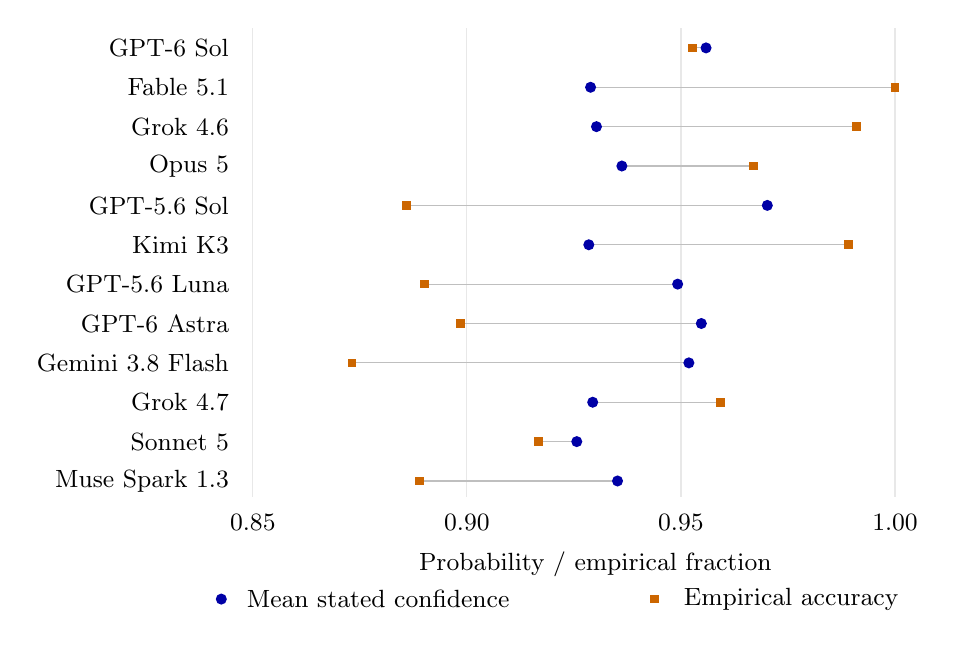
\begin{tikzpicture}[every node/.style={font=\small}]
\draw[gray!18] (0.00000,-.2)--(0.00000,5.750);
\node[anchor=north] at (0.00000,-.3) {0.85};
\draw[gray!18] (2.71875,-.2)--(2.71875,5.750);
\node[anchor=north] at (2.71875,-.3) {0.90};
\draw[gray!18] (5.43750,-.2)--(5.43750,5.750);
\node[anchor=north] at (5.43750,-.3) {0.95};
\draw[gray!18] (8.15625,-.2)--(8.15625,5.750);
\node[anchor=north] at (8.15625,-.3) {1.00};
\node[anchor=east] at (-.18,0.000) {Muse Spark 1.3};
\draw[gray!50] (4.63194,0.000)--(2.11458,0.000);
\fill[blue!65!black] (4.63194,0.000) circle (2pt);
\fill[orange!80!black] (2.05958,-0.055) rectangle (2.16958,0.055);
\node[anchor=east] at (-.18,0.500) {Sonnet 5};
\draw[gray!50] (4.11437,0.500)--(3.62500,0.500);
\fill[blue!65!black] (4.11437,0.500) circle (2pt);
\fill[orange!80!black] (3.57000,0.445) rectangle (3.68000,0.555);
\node[anchor=east] at (-.18,1.000) {Grok 4.7};
\draw[gray!50] (4.31671,1.000)--(5.93686,1.000);
\fill[blue!65!black] (4.31671,1.000) circle (2pt);
\fill[orange!80!black] (5.88186,0.945) rectangle (5.99186,1.055);
\node[anchor=east] at (-.18,1.500) {Gemini 3.8 Flash};
\draw[gray!50] (5.53798,1.500)--(1.26087,1.500);
\fill[blue!65!black] (5.53798,1.500) circle (2pt);
\fill[orange!80!black] (1.20587,1.445) rectangle (1.31587,1.555);
\node[anchor=east] at (-.18,2.000) {GPT-6 Astra};
\draw[gray!50] (5.69624,2.000)--(2.63995,2.000);
\fill[blue!65!black] (5.69624,2.000) circle (2pt);
\fill[orange!80!black] (2.58495,1.945) rectangle (2.69495,2.055);
\node[anchor=east] at (-.18,2.500) {GPT-5.6 Luna};
\draw[gray!50] (5.39567,2.500)--(2.18098,2.500);
\fill[blue!65!black] (5.39567,2.500) circle (2pt);
\fill[orange!80!black] (2.12598,2.445) rectangle (2.23598,2.555);
\node[anchor=east] at (-.18,3.000) {Kimi K3};
\draw[gray!50] (4.26726,3.000)--(7.56522,3.000);
\fill[blue!65!black] (4.26726,3.000) circle (2pt);
\fill[orange!80!black] (7.51022,2.945) rectangle (7.62022,3.055);
\node[anchor=east] at (-.18,3.500) {GPT-5.6 Sol};
\draw[gray!50] (6.53430,3.500)--(1.95559,3.500);
\fill[blue!65!black] (6.53430,3.500) circle (2pt);
\fill[orange!80!black] (1.90059,3.445) rectangle (2.01059,3.555);
\node[anchor=east] at (-.18,4.000) {Opus 5};
\draw[gray!50] (4.68704,4.000)--(6.35873,4.000);
\fill[blue!65!black] (4.68704,4.000) circle (2pt);
\fill[orange!80!black] (6.30373,3.945) rectangle (6.41373,4.055);
\node[anchor=east] at (-.18,4.500) {Grok 4.6};
\draw[gray!50] (4.36456,4.500)--(7.67076,4.500);
\fill[blue!65!black] (4.36456,4.500) circle (2pt);
\fill[orange!80!black] (7.61576,4.445) rectangle (7.72576,4.555);
\node[anchor=east] at (-.18,5.000) {Fable 5.1};
\draw[gray!50] (4.28958,5.000)--(8.15625,5.000);
\fill[blue!65!black] (4.28958,5.000) circle (2pt);
\fill[orange!80!black] (8.10125,4.945) rectangle (8.21125,5.055);
\node[anchor=east] at (-.18,5.500) {GPT-6 Sol};
\draw[gray!50] (5.75603,5.500)--(5.58229,5.500);
\fill[blue!65!black] (5.75603,5.500) circle (2pt);
\fill[orange!80!black] (5.52729,5.445) rectangle (5.63729,5.555);
\node[anchor=north] at (4.35,-.78) {Probability / empirical fraction};
\fill[blue!65!black] (-.4,-1.5) circle(2pt);\node[anchor=west] at (-.2,-1.5) {Mean stated confidence};
\fill[orange!80!black] (5.05,-1.555) rectangle(5.16,-1.445);\node[anchor=west] at (5.35,-1.5) {Empirical accuracy};\end{tikzpicture}
\caption{Conditional confidence diagnostic on predictions with $\max(p,1-p)\geq0.9$. Each row uses the subset selected by that model, rather than a common set of units. Wrong/selected counts: GPT-6 Sol: 8/169; Fable 5.1: 0/81; Grok 4.6: 1/112; Opus 5: 4/121; GPT-5.6 Sol: 26/228; Kimi K3: 1/92; GPT-5.6 Luna: 20/182; GPT-6 Astra: 21/207; Gemini 3.8 Flash: 35/276; Grok 4.7: 4/98; Sonnet 5: 5/60; Muse Spark 1.3: 15/135. This is not a full reliability diagram or an estimate of statistical significance.}\label{fig:confidence}\end{figure}

Fable has no errors among 81 high-confidence units, while Kimi and Grok 4.6 each miss one. These observations do not establish population error rates of zero or one percent. A model may achieve excellent accuracy on a smaller, easier high-confidence subset. The practical finding is that confidence behavior varies substantially and can materially affect proper scores; model price or flagship status is not a sufficient calibration guarantee.

\subsection{Inference cost}
The retained normalized successful-workload figures range from \$1.48 for GPT-5.6 Luna to \$83.18 for Fable. These are not total experiment budgets or uniform invoice charges. Fable's figure is a reconstruction of hypothetical cached execution; its historical uncached successful workload was \$189.70. Luna's billing-derived figure includes eight extra requests. Several other figures normalize provider discounts or impute missing cache information.

The retained corrected estimate for Grok 4.7 is \$33.00 at standard rates, alongside \$11.52 in provider-reported successful-call charges. Cache-adjusted pricing is not fully observed. GPT-6 Sol's corresponding standard estimate is \$11.01, versus a saved pricing-based workload estimate of \$5.50. Failed attempts and unresolved charges are generally outside these totals. On these stated estimates Luna and GPT-6 Sol form the observed cost--score frontier; its precise location depends on the accounting assumptions.

\section{A shared-summary experiment with Jev}
Jev is described by its developer as a probabilistic ``System One'' model, exposing native Boolean probabilities rather than generating an agentic legal analysis \citep{jevdocs}. Its context and interaction constraints differ from those of the document-enabled configurations. We therefore treat its evaluation as a separate experiment, not a row in the full-document model ranking.

GPT-5.6 Luna summarized each selected document using instructions to preserve material facts, arguments, authorities, and procedural posture without predicting the result. The summarizer received neither outcome labels nor other models' forecasts. Jev and two Luna comparator configurations then received the same frozen summary cache and unit questions in a single request per case, without document tools or follow-up turns. The conditions comprise Jev through the historical \texttt{typesafe-ai/jev} Gateway alias, GPT-5.6 Luna with high reasoning, and GPT-6 Luna without reasoning. The two Luna conditions differ in model generation as well as reasoning setting, so their contrast does not isolate a reasoning effect.

\begin{table}[tb]\centering\small
\begin{tabular}{lrrr}\toprule
Condition & Micro Brier & Case Brier & Acc. (\%)\\\midrule
GPT-5.6 Luna full documents & 0.14322 & 0.15084 & 80.88 \\
GPT-5.6 Luna summary + high reasoning & 0.15489 & 0.16119 & 78.55 \\
GPT-6 Luna summary + no reasoning & 0.17152 & 0.18694 & 74.16 \\
Jev summary + one-shot & 0.36754 & 0.34416 & 32.56 \\
\bottomrule\end{tabular}
\caption{Shared-summary results and the full-document Luna reference. All rows use the same 91 cases and 387 scored units. Only the last three rows share a one-request summary interface; the first row is a descriptive full-document reference.}
\label{tab:summary}\end{table}
\begin{figure}[tb]\centering
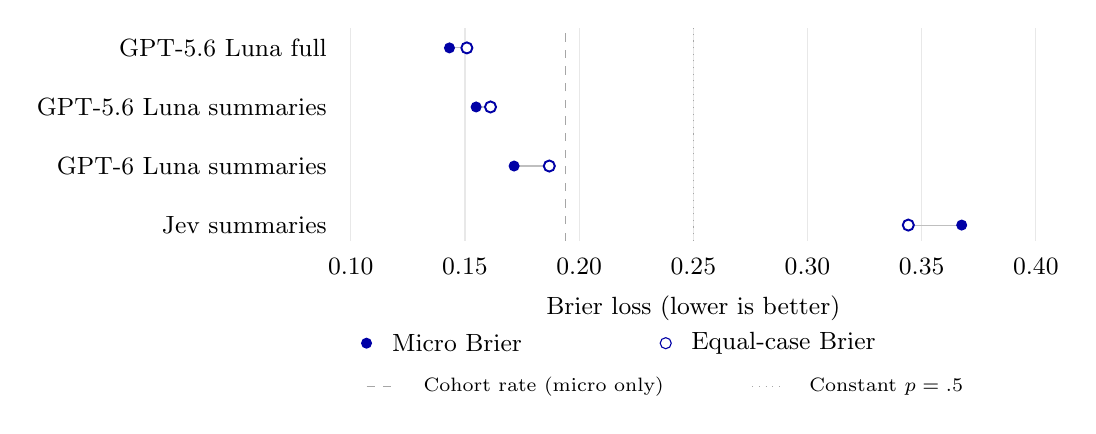
\begin{tikzpicture}[every node/.style={font=\small}]
\draw[gray!18] (0.00000,-.2)--(0.00000,2.500);
\node[anchor=north] at (0.00000,-.3) {0.10};
\draw[gray!18] (1.45000,-.2)--(1.45000,2.500);
\node[anchor=north] at (1.45000,-.3) {0.15};
\draw[gray!18] (2.90000,-.2)--(2.90000,2.500);
\node[anchor=north] at (2.90000,-.3) {0.20};
\draw[gray!18] (4.35000,-.2)--(4.35000,2.500);
\node[anchor=north] at (4.35000,-.3) {0.25};
\draw[gray!18] (5.80000,-.2)--(5.80000,2.500);
\node[anchor=north] at (5.80000,-.3) {0.30};
\draw[gray!18] (7.25000,-.2)--(7.25000,2.500);
\node[anchor=north] at (7.25000,-.3) {0.35};
\draw[gray!18] (8.70000,-.2)--(8.70000,2.500);
\node[anchor=north] at (8.70000,-.3) {0.40};
\draw[dashed,gray!70] (2.72887,-.2)--(2.72887,2.500);
\draw[dotted,gray!70] (4.35000,-.2)--(4.35000,2.500);
\node[anchor=east] at (-.18,0.000) {Jev summaries};
\draw[gray!50] (7.75870,0.000)--(7.08070,0.000);
\fill[blue!65!black] (7.75870,0.000) circle (2pt);
\draw[blue!65!black,fill=white,line width=.7pt] (7.08070,0.000) circle (2pt);
\node[anchor=east] at (-.18,0.750) {GPT-6 Luna summaries};
\draw[gray!50] (2.07411,0.750)--(2.52134,0.750);
\fill[blue!65!black] (2.07411,0.750) circle (2pt);
\draw[blue!65!black,fill=white,line width=.7pt] (2.52134,0.750) circle (2pt);
\node[anchor=east] at (-.18,1.500) {GPT-5.6 Luna summaries};
\draw[gray!50] (1.59194,1.500)--(1.77464,1.500);
\fill[blue!65!black] (1.59194,1.500) circle (2pt);
\draw[blue!65!black,fill=white,line width=.7pt] (1.77464,1.500) circle (2pt);
\node[anchor=east] at (-.18,2.250) {GPT-5.6 Luna full};
\draw[gray!50] (1.25329,2.250)--(1.47422,2.250);
\fill[blue!65!black] (1.25329,2.250) circle (2pt);
\draw[blue!65!black,fill=white,line width=.7pt] (1.47422,2.250) circle (2pt);
\node[anchor=north] at (4.35,-.78) {Brier loss (lower is better)};
\fill[blue!65!black] (.2,-1.5) circle(2pt);\node[anchor=west] at (.4,-1.5) {Micro Brier};
\draw[blue!65!black,fill=white] (4.0,-1.5) circle(2pt);\node[anchor=west] at (4.2,-1.5) {Equal-case Brier};
\draw[dashed,gray!70] (.2,-2.05)--(.6,-2.05);\node[anchor=west,font=\scriptsize] at (.8,-2.05) {Cohort rate (micro only)};\draw[dotted,gray!70] (5.1,-2.05)--(5.5,-2.05);\node[anchor=west,font=\scriptsize] at (5.7,-2.05) {Constant $p=.5$};\end{tikzpicture}
\caption{Probability quality with a shared summary cache. Both Luna conditions exploit predictive signal in the summaries, while Jev scores worse than the constant $p=0.5$ forecast. The full-document reference changes both information access and interaction. Connecting segments indicate weighting sensitivity, not uncertainty intervals.}\label{fig:summary}\end{figure}

Jev's micro-Brier of 0.36754 is worse than the 0.25 loss of always reporting $p=0.5$. Its mean predicted dismissal probability is approximately 0.305 against an observed frequency of 0.736. This directly shows severe underprediction in the aggregate, rather than inferring calibration solely from a large Brier loss. Its 32.6\% threshold accuracy is also below majority-class prediction.

GPT-5.6 Luna on the identical summaries achieves micro-Brier 0.15489 and accuracy 78.6\%. The paired case-cluster bootstrap gives a Luna-minus-Jev difference of $-0.21265$, with a 99.44\% Bonferroni-adjusted interval (95\% familywise coverage) of $[-0.32644,-0.06433]$ across the three model pairs and three metrics. The result remains exploratory because potential cross-case dependence was not assessed. The two Luna conditions are not distinguishable under this correction.

The shared-summary control shows that the summaries contain useful predictive signal that this Jev configuration does not exploit. It does not show that every material detail survived compression. Full-document Luna performs better than summary-only Luna, but that contrast changes information access and interaction together. Nor does the experiment establish that probabilistic or non-generative architectures are unsuitable for litigation. Domain exposure, task adaptation, the event formulation, and interface behavior remain possible explanations; Jev's litigation-specific training coverage is unknown.

Summary preparation cost an estimated \$10.32. Successful inference estimates are approximately \$0.044 for Jev, \$1.62 for GPT-5.6 Luna, and \$0.103 for GPT-6 Luna. These registry-based estimates exclude retries and are not invoice totals. Omitting the common preparation cost would misstate the economics of the complete pipeline.

\section{Prediction, adjudication, and legal strategy}
\label{sec:strategy}
\subsection{An observable disposition is not an infallible legal answer}
Litigation can resolve the parties' rights even when the underlying interpretation remains contestable. Holmes's contract example makes the distinction concrete: the parties anticipate different dates for a promised lecture, yet are bound by the court's construction requiring performance within a reasonable time \citep{holmes}. Finality between parties is also different from precedent governing later cases. A final, unappealed judgment on the merits can retain preclusive effect despite legal error \citep{moitie}; a ruling in one case need not settle every future application of the same rule. LegalForecastBench uses an even narrower event: the first written disposition of a specified motion. Later amendment, settlement, or appellate reversal does not alter whether that event occurred.

Politically salient constitutional disputes illustrate the difference between an authoritative decision and continuing disagreement about its correctness. Before June 24, 2022, \emph{Roe} and \emph{Casey} supplied a federal constitutional protection against certain state restrictions on abortion, including the undue-burden framework for pre-viability restrictions. In \emph{Dobbs v. Jackson Women's Health Organization}, the Supreme Court overruled those precedents and held that the federal Constitution does not confer a right to abortion \citep{dobbs}. The decision changed the governing federal constitutional rule without ending disagreement about it or resolving every issue under state constitutions and other law. For forecasting, a change of this kind also matters because past outcomes may cease to represent the legal regime governing future disputes.

\subsection{Why forecasts affect settlement}
The bargaining-in-the-shadow-of-the-law account connects expected adjudication to private agreement \citep{shadow}. A simple risk-neutral model makes the role of probability explicit \citep{shavell}. Suppose a plaintiff would receive a fixed award $J>0$ if successful and zero otherwise. Let $q_P$ and $q_D$ be the plaintiff's and defendant's respective estimates of the probability of that success, and let $k_P,k_D\geq0$ be their remaining litigation costs. Assuming each side bears its own costs, ignoring settlement costs, and restricting attention to monetary payoffs, the plaintiff's expected trial payoff is $q_PJ-k_P$, while the defendant's expected trial cost is $q_DJ+k_D$. A payment $s$ from defendant to plaintiff is weakly acceptable to both when
\begin{equation}
 q_PJ-k_P\;\leq\;s\;\leq\;q_DJ+k_D.
 \label{eq:settlement-range}
\end{equation}
The interval is nonempty when
\begin{equation}
 (q_P-q_D)J\;\leq\;k_P+k_D.
\end{equation}
This is an illustrative reservation-value calculation in the economic analysis of litigation, not an estimated model of this dataset \citep{priestklein,settlement}. Agreement about the probability of success creates a settlement surplus equal to the avoided costs. The settlement interval disappears when the plaintiff's estimate of success exceeds the defendant's estimate of the plaintiff's success by enough that $(q_P-q_D)J>k_P+k_D$. Even when the interval exists, private information or strategic bargaining can prevent agreement \citep{settlement}. A party should reject a particular settlement when its expected litigation payoff is higher under these assumptions. That does not imply that every other possible settlement is unacceptable. Nonmonetary goals, risk preferences, fee shifting, and uncertain damages require a richer model. A motion-to-dismiss probability informs this analysis but is not itself a probability of ultimate recovery or an estimate of settlement value.

\subsection{Prediction as a component of legal advice}
High-level strategic advice involves several tasks. A lawyer must (i) understand the client's objectives; (ii) analyze the documents and other facts; (iii) analyze the applicable law; (iv) predict how a court might resolve the dispute; (v) assess counterparties' incentives and objectives; (vi) identify potentially acceptable resolutions; and (vii) develop a strategy for obtaining the best realistically achievable outcome for the client. This is our decomposition of the advice task, consistent with the MacCrate skills framework and the New York State Judicial Institute's account of counseling and negotiation \citep{nylawyerskills}. Prediction informs these other activities, but does not determine the client's goals or exhaust a lawyer's professional responsibilities.

Prediction also bears on the selection and organization of arguments. Each additional point consumes briefing space and judicial attention. In \emph{Jones v. Barnes}, the Supreme Court recognized the value of selecting stronger appellate arguments and the risk that adding weaker ones can dilute them \citep{jonesbarnes}. This supports testing whether a model can prioritize consequential issues, rather than merely identify every technically available objection. A separate evaluation could ask experts to assess issue selection and the connection between the model's rationale and the court's stated grounds; forecast scores alone do not establish those abilities.

Professional experience should not be equated with demonstrated calibration. Goodman-Delahunty and colleagues' prospective study of lawyers' case-outcome predictions found overconfidence and no calibration advantage from more years in practice \citep{lawyercalibration}. The study used lawyers' own minimum case goals and reported outcomes; years of practice did not measure specialization or experience with similar disputes. The practical importance of forecasting therefore motivates measuring both human and model performance. Our study does not include a matched human baseline or a direct comparison between models' research skills and strategic judgment.

\section{Outcome feedback and LegalForecastGym}
LegalForecastGym implements a separate, single-step forecasting environment intended for post-training experiments. It renders a static litigation packet and receives a structured action containing a dismissal probability and cited evidence spans. Training loaders admit only explicitly designated training collections and reject locked test matters. Episode assembly keeps the label out of the observation. The current phase does not implement a multi-turn litigation simulator or train an agent to take procedural actions.

For a valid forecast, the implemented Brier-shaped reward is
\begin{equation}
 R(p,Y)=0.02+0.98\bigl[1-(p-Y)^2\bigr],
\end{equation}
while invalid output receives zero. The positive affine transformation preserves the proper-score optimum among valid forecasts. The implementation also supplies threshold-based and clipped-log alternatives. Evidence spans are logged rather than rewarded. This design separates a directly scored prediction from an assertion that the accompanying reasoning is legally correct.

The checked Gym artifacts contain no completed parameter-update experiment or held-out before/after training comparison. They do contain a live sampling comparison on 50 synthetic development episodes, used to assess output format and select an open-weight sampling model. That run is infrastructure evidence, not evidence of legal forecasting improvement. A separately recorded Gym export of 100 matters and 425 scoreable units is also distinct from the 91-case, 387-unit benchmark analyzed here; those populations are not pooled.

The intended learning study asks whether earlier outcome feedback improves predictions on later, disjoint matters and whether any gains extend beyond forecasting. Parameter learning, in-context feedback, and changes to the surrounding agent system are different interventions. Each needs a matched control and a held-out endpoint. Forecasting literature makes such learning plausible, and OpenForecaster reports calibration transfer to other question-answering benchmarks; those findings do not establish improved litigation strategy \citep{outcomerl,openforecaster}. Appendix~\ref{app:study} specifies a concrete prospective design.


\section{Task validity and rubric-based legal evaluation}
\subsection{Why the reward definition matters}
A June 2026 Harvey industry article characterizes litigation as slower to adopt agents than some volume-driven workflows; this is a vendor observation, not a measured cross-practice adoption study \citep{litigationAdoption}. Harvey launched LAB on May 6, 2026 as an open-source collection of legal-agent tasks with matter files, requested deliverables, and expert-written criteria \citep{harveyLAB}. The launch describes 1,200 tasks spanning 24 practice areas and more than 75,000 criteria. Its initial-results report announced a partnership with Artificial Analysis, which subsequently introduced a 120-task LAB-AA variant \citep{harveyInitial,labAA}. This establishes a prominent industry evaluation effort, not a field-wide consensus that LAB or its publisher uniquely defines legal capability.

LAB-style criteria also enter training. Harvey and Applied Compute report full-parameter reinforcement learning of a legal agent using rubric-based rewards \citep{harveyTraining}. Harvey's August 2026 Tenet research preview describes asynchronous RL of a Kimi K3-based model, with rewards combining criterion coverage, issue-level success, and perfect-completion bonuses. It reports gains on LAB and other legal benchmarks \citep{tenet}. These are first-party training reports, not independent replications, but they make task validity consequential: a misspecified reward can shape learned behavior as well as a leaderboard.

Rubrics are useful when they encode meaningful requirements and are reliably graded. The risk is a mismatch among the requested work, the record supplied, the legal answer prescribed by a criterion, and the grader's application of that criterion. These are distinct failure modes. JudgmentBench's comparison of expert rubric scores and pairwise preferences on 30 BigLaw Bench tasks provides related empirical motivation, although its constructed quality levels and task selection limit generalization \citep{judgmentbench}.

The evaluation question is one of construct validity: whether the measurements adequately represent the capability the benchmark claims to assess \citep{jacobswallach}. If the same criteria supply training rewards, a defective criterion also raises a question of reward misspecification. Reward hacking is a possible learned response to such a specification, and reward-model overoptimization is a possible divergence between an improving proxy score and the underlying target. These diagnoses require different evidence \citep{amodei,gao}. Gao and colleagues study this divergence using a synthetic gold reward model; our audit examines task and criterion validity and does not measure a training trajectory. Outcome scores also have a limited target: they reward accurate forecasts, without directly rewarding good advice or faithful explanations.

\subsection{Preliminary audit and a targeted task review}
Our retained AI-assisted review covers the pinned litigation-and-dispute-resolution subset: 52 tasks and 2,858 criteria. GPT-6 Sol flagged 616 criteria; Claude Opus 5.5's final reconciliation flagged 564. Their union contains 835 flagged criteria, leaving 2,023 unflagged by either final report. Of 345 overlapping flags, both reviewers called 83 problematic and 135 arguable; 127 received different levels of concern. The union represents 29.2\% of the 2,858 criteria; the other 70.8\% were not flagged, which does not establish that they are correct. These are review outputs, not a verified error rate. Opus's reconciliation saw Sol's findings, so agreement in the final reports is not independent confirmation \citep{labaudit}.

The author's targeted review of \texttt{analyze-counterparty-motion-to-dismiss} motivates a narrower case study (Appendix~\ref{app:lab}). Among its 34 criteria, the AI reviewers flagged 16. Source inspection supports concrete concerns: a categorical integration-clause proposition despite express non-reliance language; a required characterization of accrual as factually disputed despite dated allegations requiring careful analysis; and output requirements, including a minimum number of recommendations, that the user-facing instruction does not specify \citep{labtask}. These examples do not justify treating every flagged criterion as wrong, or treating every solver failure as a grading defect.

The task also illustrates why a realism critique must be precise. The complaint quotes a Texas forum-selection clause while filing in Georgia, but it also advances venue and scope arguments. That is a contestable litigation position, not proof that real litigants never behave this way. Similarly, the inspected motion contains a caption, table of contents, and table of authorities. Programmatic document metadata establishes templating, not LLM authorship. The strongest criticism concerns how the rubric evaluates the supplied legal problem, rather than inferring professional invalidity from the documents' appearance.

\subsection{Implications for evaluation and training}
All-pass aggregation can magnify one defective criterion: a useful work product fails if any required item fails. This does not make all-pass evaluation inherently inappropriate; some legal requirements are indispensable. It does mean that criteria should distinguish dispositive analysis, necessary completeness, and optional presentation. A benchmark should permit a well-supported rejection of a planted argument when the record or law makes that argument weak.

OpenAI's 2026 analysis of SWE-bench Verified makes an analogous concern concrete: in a selected audit of 138 difficult tasks, it reported problems involving test requirements and task specification \citep{swecritique}. That finding supports examining task--test alignment; it provides no defect estimate for LAB. Neither the preliminary LAB audit nor the present forecasting results establish that rubric-based RL is ineffective, that synthetic tasks generally harm performance, or that training on litigation tasks caused degradation. A stronger experiment would compare matched environments built from synthetic and authentic records, independently adjudicate their criteria, and evaluate transfer to held-out professional tasks.

There is also evidence that rubric-based training can improve performance under a different evaluation format. Gunjal and colleagues report gains on GPQA-Diamond, a multiple-choice science benchmark, relative to direct Likert-based judge rewards \citep{rubricsrewards}. This result does not establish transfer to legal tasks, but it cautions against assuming that rubric rewards merely teach compliance with the training rubric.

Real litigation is valuable because it supplies naturally occurring arguments, procedural complexity, and an outcome that the benchmark designer did not choose. It still requires expert construction. Authentic records can support both outcome scoring and carefully validated rubrics. The research opportunity is to test which supervision signals teach useful judgment, rather than assuming that either the court's outcome or an expert checklist is a complete measure of legal competence.

\paragraph{Industry use and the limits of that evidence.} Harvey's product announcements report LAB all-pass results for Opus 4.8 (10.4\%, May 28), Fable 5 (13.3\%, June 9), and Sonnet 5 (5.8\%, June 30) \citep{opusAnnouncement,fableAnnouncement,sonnetAnnouncement}. These examples show repeated use in model evaluation and product positioning. They are Harvey's evaluations of third-party models, not evidence that each model developer independently adopted LAB as its definitive legal benchmark. The LAB-AA partnership broadens distribution, but neither prominence nor a commercial partnership establishes evaluation validity.


\section{Limitations and generalization}
\paragraph{Selection into adjudication.} The target population is a set of accessible cases with written motion decisions, not all disputes, all filed cases, or all contemplated motions. Parties settle, abandon claims, amend pleadings, or choose not to sue. Cases reaching a published disposition may differ in uncertainty, stakes, representation, and bargaining conditions. Calibration conditional on reaching this dataset does not establish calibration for counterfactual outcomes in the broader dispute population \citep{priestklein}. At the same time, selection does not prove that learned skills cannot transfer: that is an empirical question requiring an independently defined evaluation population.

\paragraph{Prediction is not legal correctness.} Judicial outcomes reflect doctrine and record facts, but also procedure, judicial behavior, and institutional context. Judge identity remains visible. We have not established how much performance comes from close legal analysis rather than judge, court, party, or case-type priors. A metadata-only comparison, judge masking, and a human forecasting baseline are important future tests. Neither fluent rationales nor a correct forecast demonstrate valid legal reasoning. Training to imitate outcomes can reproduce historical disparities or errors; professional advice also has obligations that prediction scores do not capture.

\paragraph{Labels and completeness.} Unitization can omit, merge, or split legally distinct targets; dispositions can be ambiguous or procedural. Human oversight helps but does not quantify residual error. The absence of a complete blinded label audit and acquisition/exclusion census limits claims about both label accuracy and representativeness. Excluding 22 unscored units preserves an interpretable target but may also change difficulty. These limitations deserve the same scrutiny as disputed rubrics in another benchmark.

\paragraph{Statistical and execution limits.} One retained successful prediction per unit does not characterize run-to-run variance, operational reliability, or expected total cost. The cohort is small and imbalanced. Case clustering does not resolve unverified dependence among related cases. Incomplete local recovery of seven models' per-unit inputs limits reanalysis. Reported scores compare model--harness--provider configurations, not isolated model weights.

\paragraph{Temporal and transfer limits.} A provider-reported cutoff and disabled browsing reduce specific leakage risks without proving contamination absent. New benchmark versions change the case distribution. Generalization to other jurisdictions, procedural stages, settlement decisions, drafting, or strategic advice is not established by this study. Outcome feedback may improve a narrow probability estimate without improving explanations or real client decisions.

\section{Conclusion}
LegalForecastBench operationalizes an uncertain but consequential legal judgment as a probabilistic forecast of a later judicial event. In the beta, all twelve document-enabled configurations outperform a cohort-fitted constant in micro-Brier, while confidence behavior and model ordering differ in informative ways. GPT-6 Sol has the strongest observed scores, and the shared-summary comparison exposes a large gap between Jev and Luna that cannot be explained by the summaries containing no signal.

The broader opportunity is to make legal evaluation more empirically grounded. Real outcomes provide an external scoring reference, but useful training signals still require careful task definition, information boundaries, and legal labeling. The next research question is whether feedback on such forecasts improves performance on later cases and transfers to independently assessed legal work. The present evidence motivates that question; it does not answer it.

\section*{Reproducibility, access, and disclosure}
This manuscript preserves the twelve-configuration panel in the supplied working draft and checks its numerical claims against the retained repository artifacts as of September 29, 2026. The accompanying aggregate data and figure script regenerate the plots without court-document bytes. Code and result artifacts are maintained in the \href{https://github.com/johnhughes3/LegalForecastBench}{LegalForecastBench repository}; access to restricted source documents and private adjudication material is a separate audit process. Availability of code is not equivalent to unrestricted source-data replication.

The author designed the benchmark and supplied domain judgments. AI assistants supported this manuscript's drafting, literature retrieval, and numerical and source checks. The LAB audit discussed below is explicitly an AI-assisted preliminary analysis; the author's targeted task review is distinguished from a completed independent audit. No model-weight reinforcement-learning experiment is claimed unless explicitly identified as a result of an external cited study.

\clearpage

\begin{thebibliography}{99}

\bibitem{deepseek} Daya Guo, Dejian Yang, Haowei Zhang et al. DeepSeek-R1 incentivizes reasoning in LLMs through reinforcement learning. \emph{Nature 645, 633--638 (2025); arXiv:2501.12948v2}, 2025. \url{https://www.nature.com/articles/s41586-025-09422-z}.

\bibitem{rlve} Zhiyuan Zeng, Hamish Ivison, Yiping Wang et al. RLVE: Scaling Up Reinforcement Learning for Language Models with Adaptive Verifiable Environments. \emph{ICML 2026, Proceedings of Machine Learning Research 306:153406--153428}, 2026. \url{https://proceedings.mlr.press/v306/zeng26j.html}.

\bibitem{alphazero} David Silver, Thomas Hubert, Julian Schrittwieser et al. Mastering Chess and Shogi by Self-Play with a General Reinforcement Learning Algorithm. \emph{arXiv:1712.01815 (2017), preprint; precursor to the distinct 2018 Science article}, 2017. \url{https://arxiv.org/abs/1712.01815}.

\bibitem{alphaproof} Thomas Hubert, Rishi Mehta, Laurent Sartran et al. Olympiad-level formal mathematical reasoning with reinforcement learning. \emph{Nature 651, 607--613; version of record 13 March 2026}, 2026. \url{https://www.nature.com/articles/s41586-025-09833-y}.

\bibitem{navierstokesproof} OpenAI. Finite Time Blowup for Navier--Stokes. \emph{Technical manuscript}, September 2026. \url{https://cdn.openai.com/pdf/32d9f210-8b73-45e0-91bc-82a30aef8a9a/navier-stokes.pdf}.

\bibitem{navierstokesreport} OpenAI. On the Navier--Stokes Millennium Prize Problem. \emph{Research announcement}, September 8, 2026; updated September 10, 2026. \url{https://openai.com/index/navier-stokes-solution/}.

\bibitem{judgmentbench} Russell Yang, Ruishi Chen, Pierce Kelaita et al. JudgmentBench: Comparing Rubric and Preference Evaluation for Quality Assessment. \emph{arXiv:2605.25240v3, preprint}, 2026. \url{https://arxiv.org/abs/2605.25240}.

\bibitem{rubricsrewards} Anisha Gunjal, Anthony Wang, Elaine Lau, Vaskar Nath, Yunzhong He, Bing Liu, and Sean Hendryx. Rubrics as Rewards: Reinforcement Learning Beyond Verifiable Domains. In \emph{International Conference on Learning Representations}, 2026. First posted as arXiv:2507.17746 in 2025. \url{https://proceedings.iclr.cc/paper_files/paper/2026/hash/cfd7bee7a651ee9af525098ef67a9e45-Abstract-Conference.html}.

\bibitem{harveyTraining} Niko Grupen, Julio Pereyra, Gabe Pereyra et al. Training a Legal Agent with Applied Compute. \emph{Primary online source}, 2026. \url{https://www.harvey.ai/blog/training-a-legal-agent-with-applied-compute}.

\bibitem{tenet} Calvin Qi, Vasudha Rengarajan, Julio Pereyra et al. Harvey Tenet Research Preview. \emph{August 20, 2026 company research report}, 2026. \url{https://www.harvey.ai/blog/post-training-update-harvey-tenet}.

\bibitem{instructgpt} Long Ouyang, Jeffrey Wu, Xu Jiang et al. Training language models to follow instructions with human feedback. \emph{NeurIPS 2022}, 2022. \url{https://arxiv.org/abs/2203.02155}.

\bibitem{legalbench} Neel Guha, Julian Nyarko, Daniel E. Ho et al. LegalBench: A Collaboratively Built Benchmark for Measuring Legal Reasoning in Large Language Models. \emph{NeurIPS 2023, Datasets and Benchmarks}, 2023. \url{https://arxiv.org/abs/2308.11462}.

\bibitem{ncbe} National Conference of Bar Examiners. About the Multistate Bar Examination. Official examination description, n.d.; accessed September 29, 2026. \url{https://www.ncbex.org/exams/mbe/about-mbe}.

\bibitem{hart} H. L. A. Hart. Positivism and the Separation of Law and Morals. \emph{Harvard Law Review}, 71(4):593--629, 1958. Especially pp. 607--608. \url{https://www.jstor.org/stable/1338225}.

\bibitem{fuller} Lon L. Fuller. Positivism and Fidelity to Law---A Reply to Professor Hart. \emph{Harvard Law Review}, 71(4):630--672, 1958. Especially pp. 661--664. \url{https://www.jstor.org/stable/1338226}.

\bibitem{declaratory} United States Congress. Declaratory Judgment Act, 28 U.S.C.\ \S\ 2201(a). Text consulted September 29, 2026. \url{https://www.law.cornell.edu/uscode/text/28/2201}.

\bibitem{moitie} Supreme Court of the United States. Federated Department Stores, Inc. v. Moitie, 452 U.S.\ 394, 398--399 (1981). \url{https://www.govinfo.gov/content/pkg/USREPORTS-452/pdf/USREPORTS-452-394.pdf}.

\bibitem{brier} Glenn W. Brier. Verification of Forecasts Expressed in Terms of Probability. \emph{Monthly Weather Review 78(1) (1950), 1--3}, 1950. \url{https://journals.ametsoc.org/view/journals/mwre/78/1/1520-0493_1950_078_0001_vofeit_2_0_co_2.xml}.

\bibitem{gneiting} Tilmann Gneiting, Adrian E. Raftery. Strictly Proper Scoring Rules, Prediction, and Estimation. \emph{Journal of the American Statistical Association 102 (2007), 359--378}, 2007. \url{https://doi.org/10.1198/016214506000001437}.

\bibitem{holmes} Oliver Wendell Holmes, Jr. The Path of the Law. \emph{Harvard Law Review}, 10(8):457--478, 1897. Especially pp. 457, 460--461. \url{https://www.jstor.org/stable/1322028}.

\bibitem{shadow} Robert H. Mnookin and Lewis Kornhauser. Bargaining in the Shadow of the Law: The Case of Divorce. \emph{Yale Law Journal}, 88(5):950--997, 1979. \url{https://doi.org/10.2307/795824}.

\bibitem{nylawyerskills} Paul C. Saunders. Legal Skills and Professional Values: A Handbook. \emph{Journal of the New York State Judicial Institute on Professionalism in the Law}, 7(1), Fall 2019. Reproducing and discussing the MacCrate skills framework. \url{https://www.nycourts.gov/LegacyPDFS/ip/JIPL/pdf/JIPL%20-%20FINAL%20-%20Skills%20and%20Professional%20Values.pdf}.

\bibitem{outcomerl} Benjamin Turtel, Danny Franklin, Kris Skotheim et al. Outcome-based Reinforcement Learning to Predict the Future. \emph{Transactions on Machine Learning Research (November 2025); arXiv:2505.17989v4}, 2025. \url{https://arxiv.org/abs/2505.17989}.

\bibitem{openforecaster} Nikhil Chandak, Shashwat Goel, Ameya Prabhu et al. Scaling Open-Ended Reasoning To Predict the Future. \emph{arXiv:2512.25070v2 (January 2026); preprint}, 2026. \url{https://arxiv.org/abs/2512.25070}.

\bibitem{sentencing} Junjie Chen, Haitao Li, Qilei Zhang et al. Multi-Source Retrieval and Reasoning for Legal Sentencing Prediction. \emph{arXiv:2602.04690v3; arXiv record comments 'EMNLP 2026 main' (publisher proceedings record not independently checked)}, 2026. \url{https://arxiv.org/abs/2602.04690}.

\bibitem{labaudit} GPT-6 Sol audit workers, Claude Opus 5.5 audit workers, Coordinating agents; individual provenance not fully recorded. Harvey LAB litigation and dispute resolution audit: GPT-6 Sol and Claude Opus 5.5. \emph{Local research artifact, pinned September 29, 2026}, 2026. \url{https://github.com/johnhughes3/LegalForecastBench/tree/58371a0e13494e591710e2eae3da8e428eebc359/docs/harvey-lab-audit/litigation-dispute-resolution}.

\bibitem{labtask} Harvey AI task authors; upstream authorship not individually listed. Pinned LAB task.json for analyze-counterparty-motion-to-dismiss. \emph{Primary online source}, 2026. \url{https://github.com/harveyai/harvey-labs/blob/1dd81403b2fbb60596f7aea3fcecafad7bf73143/tasks/litigation-dispute-resolution/analyze-counterparty-motion-to-dismiss/task.json}.

\bibitem{jacobswallach} Abigail Z. Jacobs and Hanna Wallach. Measurement and Fairness. In \emph{Proceedings of the 2021 ACM Conference on Fairness, Accountability, and Transparency}, pp. 375--385, 2021. \url{https://doi.org/10.1145/3442188.3445901}.

\bibitem{amodei} Dario Amodei, Chris Olah, Jacob Steinhardt, Paul Christiano, John Schulman, and Dan Man\'e. Concrete Problems in AI Safety. \emph{arXiv:1606.06565v2}, 2016. \url{https://arxiv.org/abs/1606.06565}.

\bibitem{gao} Leo Gao, John Schulman, and Jacob Hilton. Scaling Laws for Reward Model Overoptimization. In \emph{Proceedings of the 40th International Conference on Machine Learning}, PMLR 202:10835--10866, 2023. \url{https://proceedings.mlr.press/v202/gao23h.html}.

\bibitem{ruger} Theodore W. Ruger, Pauline T. Kim, Andrew D. Martin, Kevin M. Quinn. The Supreme Court Forecasting Project: Legal and Political Science Approaches to Predicting Supreme Court Decision-Making. \emph{Columbia Law Review 104 (2004), 1150--1210}, 2004. \href{https://andrewdmartin.wustl.edu/app/uploads/2019/01/The-Supreme-Court-Forecasting-Project-Legal-and-Political-Science-Approaches-to-Predicting-Supreme-Court-Decision-Making-2bvpcdb.pdf}{Author-hosted article PDF}.

\bibitem{katz} Daniel Martin Katz, Michael J. Bommarito II, Josh Blackman. A General Approach for Predicting the Behavior of the Supreme Court of the United States. \emph{PLOS ONE 12(4): e0174698 (2017)}, 2017. \url{https://journals.plos.org/plosone/article?id=10.1371%2Fjournal.pone.0174698}.

\bibitem{aletras} Nikolaos Aletras, Dimitrios Tsarapatsanis, Daniel Preotiuc-Pietro, Vasileios Lampos. Predicting Judicial Decisions of the European Court of Human Rights: A Natural Language Processing Perspective. \emph{PeerJ Computer Science 2:e93 (2016)}, 2016. \url{https://peerj.com/articles/cs-93/}.

\bibitem{cail} Chaojun Xiao, Haoxi Zhong, Zhipeng Guo et al. CAIL2018: A Large-Scale Legal Dataset for Judgment Prediction. \emph{arXiv:1807.02478 (2018); CAIL challenge dataset paper}, 2018. \url{https://arxiv.org/abs/1807.02478}.

\bibitem{medvedeva} Masha Medvedeva, Pauline McBride. Legal Judgment Prediction: If You Are Going to Do It, Do It Right. \emph{Proceedings of the Natural Legal Language Processing Workshop (ACL), 2023, pp. 73--84}, 2023. \url{https://aclanthology.org/2023.nllp-1.9/}.

\bibitem{clcuket} Huiyuan Xie, Felix Steffek, Joana Ribeiro de Faria et al. The CLC-UKET Dataset: Benchmarking Case Outcome Prediction for the UK Employment Tribunal. \emph{Proceedings of the Natural Legal Language Processing Workshop (ACL), 2024, pp. 81--96}, 2024. \url{https://aclanthology.org/2024.nllp-1.7/}.

\bibitem{harveyLAB} Niko Grupen, Gabe Pereyra, Julio Pereyra. Introducing Harvey's Legal Agent Benchmark. \emph{Primary online source}, 2026. \url{https://www.harvey.ai/blog/introducing-harveys-legal-agent-benchmark}.

\bibitem{lightman} Hunter Lightman, Vineet Kosaraju, Yura Burda et al. Let's Verify Step by Step. \emph{ICLR 2024; arXiv:2305.20050}, 2024. \url{https://arxiv.org/abs/2305.20050}.

\bibitem{autocast} Andy Zou, Tristan Xiao, Ryan Jia et al. Forecasting Future World Events with Neural Networks. \emph{NeurIPS 2022, Datasets and Benchmarks}, 2022. \url{https://arxiv.org/abs/2206.15474}.

\bibitem{halawi} Danny Halawi, Fred Zhang, Chen Yueh-Han, Jacob Steinhardt. Approaching Human-Level Forecasting with Language Models. \emph{ICML 2024, Proceedings of Machine Learning Research 235}, 2024. \url{https://arxiv.org/abs/2402.18563}.

\bibitem{forecastbench} Ezra Karger, Houtan Bastani, Chen Yueh-Han et al. ForecastBench: A Dynamic Benchmark of AI Forecasting Capabilities. \emph{ICLR2025}, 2025. \url{https://arxiv.org/abs/2409.19839}.

\bibitem{miller} Evan Miller. Adding Error Bars to Evals: A Statistical Approach to Language Model Evaluations. \emph{arXiv preprint}, 2024. \url{https://arxiv.org/abs/2411.00640}.

\bibitem{swebench} Carlos E. Jimenez, John Yang, Alexander Wettig et al. SWE-bench: Can Language Models Resolve Real-World GitHub Issues?. \emph{ICLR 2024}, 2024. \url{https://arxiv.org/abs/2310.06770}.

\bibitem{swecritique} OpenAI. Why SWE-bench Verified no longer measures frontier coding capabilities. \emph{Primary online source}, 2026. \url{https://openai.com/index/why-we-no-longer-evaluate-swe-bench-verified/}.

\bibitem{jevdocs} TypeSafe AI. Models: Jev and the System One Interface. \emph{Product documentation, accessed September 29, 2026}, 2026. \url{https://docs.typesafe.ai/models}.

\bibitem{dobbs} Supreme Court of the United States. Dobbs v. Jackson Women's Health Organization, 597 U.S.\ 215 (2022). Decided June 24, 2022. \url{https://www.supremecourt.gov/opinions/21pdf/19-1392_6j37.pdf}.

\bibitem{shavell} Steven Shavell. Economic Analysis of Litigation and the Legal Process. \emph{NBER Working Paper 9697}, 2003. Chapter 17 of the draft \emph{Foundations of Economic Analysis of Law}. \url{https://www.nber.org/papers/w9697}.

\bibitem{priestklein} George L. Priest, Benjamin Klein. The Selection of Disputes for Litigation. \emph{Journal of Legal Studies 13 (1984), 1--55}, 1984. \url{https://www.journals.uchicago.edu/doi/10.1086/467732}.

\bibitem{settlement} Lucian A. Bebchuk. Litigation and Settlement Under Imperfect Information. \emph{RAND Journal of Economics 15(3) (1984), 404--415}, 1984. \url{https://hls.harvard.edu/bibliography/litigation-and-settlement-under-imperfect-information/}.

\bibitem{jonesbarnes} Supreme Court of the United States. Jones v. Barnes, 463 U.S.\ 745, 751--753 (1983). \url{https://tile.loc.gov/storage-services/service/ll/usrep/usrep463/usrep463745/usrep463745.pdf}.

\bibitem{lawyercalibration} Jane Goodman-Delahunty, P\"ar Anders Granhag, Maria Hartwig, and Elizabeth F. Loftus. Insightful or Wishful: Lawyers' Ability to Predict Case Outcomes. \emph{Psychology, Public Policy, and Law}, 16(2):133--157, 2010. \url{https://doi.org/10.1037/a0019060}.

\bibitem{litigationAdoption} Harvey Team. How AI Agents are Changing the Way Lawyers do Legal Work. \emph{Primary online source}, 2026. \url{https://www.harvey.ai/blog/ai-agents-for-legal-work}.

\bibitem{harveyInitial} Niko Grupen, Gabe Pereyra, Julio Pereyra. Legal Agent Benchmark: Initial Results. \emph{Primary online source}, 2026. \url{https://www.harvey.ai/blog/legal-agent-benchmark-initial-results}.

\bibitem{labAA} Artificial Analysis. Harvey LAB-AA: New Benchmark Evaluating AI on Legal Tasks. \emph{July 7, 2026, benchmark announcement}, 2026. \url{https://artificialanalysis.ai/articles/harvey-lab-aa}.

\bibitem{opusAnnouncement} Harvey Team. Opus 4.8, Now Live in Harvey. \emph{Primary online source}, 2026. \url{https://www.harvey.ai/blog/opus-4-8-now-live-in-harvey}.

\bibitem{fableAnnouncement} Harvey Team. Fable 5, Now Available in Harvey. \emph{Primary online source}, 2026. \url{https://www.harvey.ai/blog/fable-5-now-available-in-harvey}.

\bibitem{sonnetAnnouncement} Harvey Team. Claude Sonnet 5, Now Live in Harvey. \emph{Primary online source}, 2026. \url{https://www.harvey.ai/blog/sonnet-5-in-harvey}.

\bibitem{atlantic} United States Supreme Court. Atlantic Marine Construction Co. v. United States District Court. \emph{571 U.S.49,59--66 (2013)}, 2013. \url{https://www.law.cornell.edu/supremecourt/text/12-929}.

\bibitem{texasLimitations} Texas Legislature. Texas Civil Practice and Remedies Code, Chapter 16. \emph{Texas Civil Practice and Remedies Code § 16.070, accessed September 29, 2026}, 2026. \url{https://statutes.capitol.texas.gov/Docs/CP/htm/CP.16.htm#16.070}.

\bibitem{jones} Supreme Court of the United States. Jones v. Bock. \emph{549 U.S.199,215}, 2007. \url{https://tile.loc.gov/storage-services/service/ll/usrep/usrep549/usrep549199/usrep549199.pdf}.

\bibitem{italiancowboy} Supreme Court of Texas. Italian Cowboy Partners, Ltd. v. Prudential Insurance Co. of America. \emph{341 S.W.3d 323, 334--37 (Tex. 2011)}, 2011. \url{https://www.txcourts.gov/media/819896/OpinionsFY2011.pdf}.

\bibitem{claynavierstokes} Clay Mathematics Institute. Navier--Stokes Announcement. September 11, 2026. \url{https://www.claymath.org/news/navier-stokes-announcement/}.

\end{thebibliography}

\clearpage

\appendix
\section{Model configuration and temporal evidence}
\label{app:cutoffs}\label{app:protocol}
The table records the maintained local evidence, rather than certifying provider training histories. ``K'' denotes a reported knowledge cutoff, ``T'' a reported training cutoff, and ``?'' no established cutoff. Month-only dates are conservatively treated as month-end. The reported cutoffs for nine configurations precede June 30, 2026. Fable, Kimi, and Muse remain qualified. A release date is not used to fill an unknown cutoff.
\begin{table}[ht]\centering\small\setlength{\tabcolsep}{4pt}
\begin{tabular}{llll}\toprule
Configuration & Reasoning & Reported cutoff & Relation to window\\\midrule
GPT-6 Sol & High & 2026-04-20 (K) & Precedes window \\
Claude Fable 5.1 & Adaptive/default & 2026-06 (T) & Possible overlap \\
Grok 4.6 & High & 2026-02-01 (K) & Precedes window \\
Claude Opus 5 & Adaptive/default & 2026-05 (T) & Precedes window \\
GPT-5.6 Sol & High & 2026-02-16 (K) & Precedes window \\
Kimi K3 & High & Unknown (?) & Unknown \\
GPT-5.6 Luna & High & 2026-02-16 (K) & Precedes window \\
GPT-6 Astra & High & 2026-04-30 (K) & Precedes window \\
Gemini 3.8 Flash & High thinking & 2026-03 (K) & Precedes window \\
Grok 4.7 & High & 2026-05 (K) & Precedes window \\
Claude Sonnet 5 & Adaptive/default & 2026-01 (T) & Precedes window \\
Muse Spark 1.3 & High & Unknown (?) & Unknown \\
\bottomrule\end{tabular}\caption{Configuration and cutoff evidence retained by the benchmark. ``Precedes window'' is a date comparison under the maintained rule, not an independently verified training-history claim.}\label{tab:cutoffs}\end{table}

The common document interface standardizes access, not every inference setting. Claude configurations use adaptive thinking at provider defaults; the others use the high reasoning or thinking setting recorded in their registries. Provider-default sampling and serving updates may still introduce variation. Full-document predictions and the one-request shared-summary conditions are kept separate throughout the analysis.

\section{Result provenance and scope of numerical reproduction}
The primary cohort identifier is \texttt{cycle-1-91-2026-09-08-luna-r5}. The ten historical aggregate rows are retained in the September 18 beta snapshot. GPT-6 Sol and Grok 4.7 are added from their native scored exports. The corrected Grok 4.7 cost comes from the receipt-cost reconstruction; it changes the cost estimate, not its forecast scores.

For this manuscript, unit-level score arithmetic can be recomputed for GPT-6 Sol, Grok 4.7, GPT-5.6 Sol, Claude Opus 5, and Claude Sonnet 5, and for all three summary conditions. The other seven main-panel rows are checked against the retained published aggregate rather than independently rederived from forecasts. The distinction is material for full-panel uncertainty and log-loss claims. The original ten-model bootstrap is reported as retained historical analysis. We independently reran the complete shared-summary comparison with one million paired case resamples and reproduced all nine retained pair-by-metric intervals exactly.

\begin{table}[ht]\centering\small
\begin{tabular}{p{.31\linewidth}p{.60\linewidth}}\toprule
Artifact & What was checked\\\midrule
Historical ten-model snapshot & Aggregate scores, cohort counts, confidence counts, historical bootstrap scope.\\
Five available main-panel unit exports & Recomputed micro Brier, equal-case Brier, and threshold accuracy.\\
Three summary-condition unit exports & Recomputed all scores and the complete million-resample, nine-comparison bootstrap.\\
LAB pinned snapshot & 52 tasks, 2,858 criteria; final flag overlap; selected task JSON and source documents.\\
Gym source and retained experiment records & Reward implementation and split controls; no completed parameter-update study found.\\
\bottomrule\end{tabular}\caption{Numerical and methodological verification performed for this manuscript. Aggregate checking and unit-level recomputation are different forms of evidence.}\end{table}

The checked source revisions are \href{https://github.com/johnhughes3/LegalForecastBench/tree/58371a0e13494e591710e2eae3da8e428eebc359}{LegalForecastBench \texttt{58371a0e}}, LegalForecastCorpus \texttt{b392ddaf}, and LegalForecastGym \texttt{4cc0f528}. The LAB source snapshot is \href{https://github.com/harveyai/harvey-labs/tree/1dd81403b2fbb60596f7aea3fcecafad7bf73143}{\texttt{1dd81403}}. These identify inspected versions; they do not certify every historical execution against the current source tree.


\section{A bounded LAB motion-to-dismiss case study}
\label{app:lab}
This case study uses the task and supplied documents at the pinned upstream revision recorded by the local audit. The requested output is an opposition issues memorandum. The fictional dispute concerns a software-services agreement, alleged pre-contractual representations, implementation defects, and a motion asserting jurisdictional, venue, and pleading defenses. We distinguish direct record observations from legal interpretations and unverified AI flags.

\paragraph{Forum selection and litigation strategy.} Complaint paragraph 48 sets out a clause selecting state or federal courts in Travis County, Texas, while the action is filed in the Northern District of Georgia. Paragraphs 18--19 assert statutory venue in Georgia, and paragraph 123 argues that the statutory deceptive-practices claim falls outside the clause. Those arguments may be weak, but the complaint is not wholly silent about the forum issue. A rigorous task should ask whether transfer is likely, which claims the clause covers, and whether a procedural objection changes the client's position. Under \emph{Atlantic Marine}, a valid clause selecting another federal forum is generally enforced through section 1404(a), while a state or foreign forum implicates forum non conveniens \citep{atlantic}. Correcting an opponent's procedural vehicle is not the same as establishing that the chosen Georgia forum will retain the dispute. A criterion that emphasizes the former without measuring the latter can reward issue identification without strategic assessment.

\paragraph{Accrual and pleaded dates.} Criteria C-013--C-015 require an accrual dispute and alternative discovery dates. The complaint alleges discovery of integration problems in August 2022, latency problems by November 2022, an acknowledgment in January 2023, and an unsuccessful patch on April 15, 2023. Paragraph 83 alleges that the plaintiff could not know the full extent of the breach until the patch failed, claims reliance on a promised fix, and states a March 22, 2024 filing date. These allegations require analyzing knowledge sufficient for accrual, distinct breaches, tolling or estoppel, and enforceability of the one-year contract term. Texas law itself restricts contractual limitations periods, subject to statutory exceptions \citep{texasLimitations}.

The appropriate critique is therefore not that the dates mechanically prove the entire claim time-barred. Nor is it enough to announce that knowledge is always a fact issue immune from dismissal. A plaintiff's allegations can establish an affirmative defense on the face of the pleading, while a genuine factual or legal issue may prevent that result \citep{jones}. The rubric should require applying the governing rule to the actual chronology and contract. It should allow the model to distinguish stronger from weaker opposition arguments instead of requiring the conclusion that every accrual question is unresolved.

\paragraph{Integration versus non-reliance.} Criterion C-012 requires the model to characterize the merger-clause defense as legally incorrect. MSA section 14.7 also contains express non-reliance language, which is analytically distinct from an ordinary integration clause. Texas authority distinguishes these contractual concepts and examines the language and surrounding circumstances \citep{italiancowboy}. The source record therefore does not justify a categorical rubric requiring the ordinary-merger-clause answer without that analysis. This observation identifies an overbroad criterion; it does not establish that the particular disclaimer is enforceable or that the fraud claim must fail.

\paragraph{Hidden output requirements.} C-028 requires concrete opposition recommendations for at least eight issues, although the prompt supplies no minimum count. C-022--C-025 prescribe high-severity treatment of specified issues. These criteria permit equivalent severity language; it would be inaccurate to say they necessarily require literal labels. C-026 prescribes organization tied to the motion's framework and expressly permits omitting Rule 12(b)(1) when no genuine issue exists. Whether those requirements improve usefulness to counsel is a measurement question. They should not be confused with independently established legal errors.

\paragraph{Document construction and limits of the review.} The supplied documents have programmatic-generation metadata and include a stale table-of-contents instruction in the agreement. The motion nevertheless has recognizable filing components. We have not established a court-rule violation warranting striking it, proven LLM authorship, or estimated how often such artifacts occur across LAB. Synthetic design can be useful for controlled testing; the concern is whether the rewarded conduct transfers to actual matters. The local audit also records genuine solver mistakes and unresolved legal disagreements. A benchmark-wide conclusion would require a representative expert review of source documents, criteria, model outputs, and grading decisions.


\section{A prospective test of outcome feedback}
\label{app:study}
A follow-up would freeze a base model and an earlier training cohort, then compare outcome feedback with a matched control on later, disjoint cases. Related cases should remain together across splits. The primary endpoint would be a predeclared difference in proper score; calibration, failure rates, cost, and reasoning validity would be secondary endpoints. Blinded expert assessment of advice or drafting would test transfer.

For a model emitting a rationale $z$ and forecast $p$, a candidate objective is
\begin{equation}
 \max_\theta\;\mathbb E_{(X,U,Y)\sim\mathcal D_{\mathrm{train}},\,(z,p)\sim\pi_\theta(\cdot\mid X,U)}\left[1-(p-Y)^2\right].
\end{equation}
This is an outcome-scored prediction objective, not a simulator that allows the agent to alter the litigation trajectory. Optimizing it need not require reinforcement learning: supervised probabilistic prediction, calibration, and policy-gradient approaches are competing methods to test. It also does not directly reward faithful rationales. Leakage-controlled held-out cases and an independent transfer endpoint are therefore necessary to distinguish generalization from memorized case outcomes or improved probability reporting alone.



\end{document}
